\documentclass[problem]{mcs}

\begin{pcomments}
  \pcomment{from: S09.cp3r}
  \pcomment{There is some pdf error that needs to be addressed}
%  \pcomment{}
\end{pcomments}

\pkeywords{
  relations
  scheduling
  partial_orders
}

%%%%%%%%%%%%%%%%%%%%%%%%%%%%%%%%%%%%%%%%%%%%%%%%%%%%%%%%%%%%%%%%%%%%%
% Problem starts here
%%%%%%%%%%%%%%%%%%%%%%%%%%%%%%%%%%%%%%%%%%%%%%%%%%%%%%%%%%%%%%%%%%%%%

\begin{problem}

\bparts

\ppart\label{prereqtable}
Draw a diagram of the prerequisite relation among MIT subjects given by
this table:
\begin{center}
\begin{tabular}{|l|l|}
\hline
Direct Prerequisites & Subject\\ \hline
 18.01 & 6.042\\ \hline
 18.01 & 18.02\\ \hline
 18.01 & 18.03\\ \hline
 8.01  & 8.02\\ \hline
 8.01  & 6.01\\ \hline
 6.042 & 6.046\\ \hline
 18.02, 18.03, 8.02, 6.01 & 6.02\\ \hline
 6.01, 6.042 & 6.006\\ \hline
 6.01 & 6.034\\ \hline
 6.02 & 6.004\\ \hline
\end{tabular}
\end{center}

\TBA{fix error in pdf attachment...}

\begin{solution}
See attached.
\iffalse
%Causes some kind of pdf version error;

\begin{center}
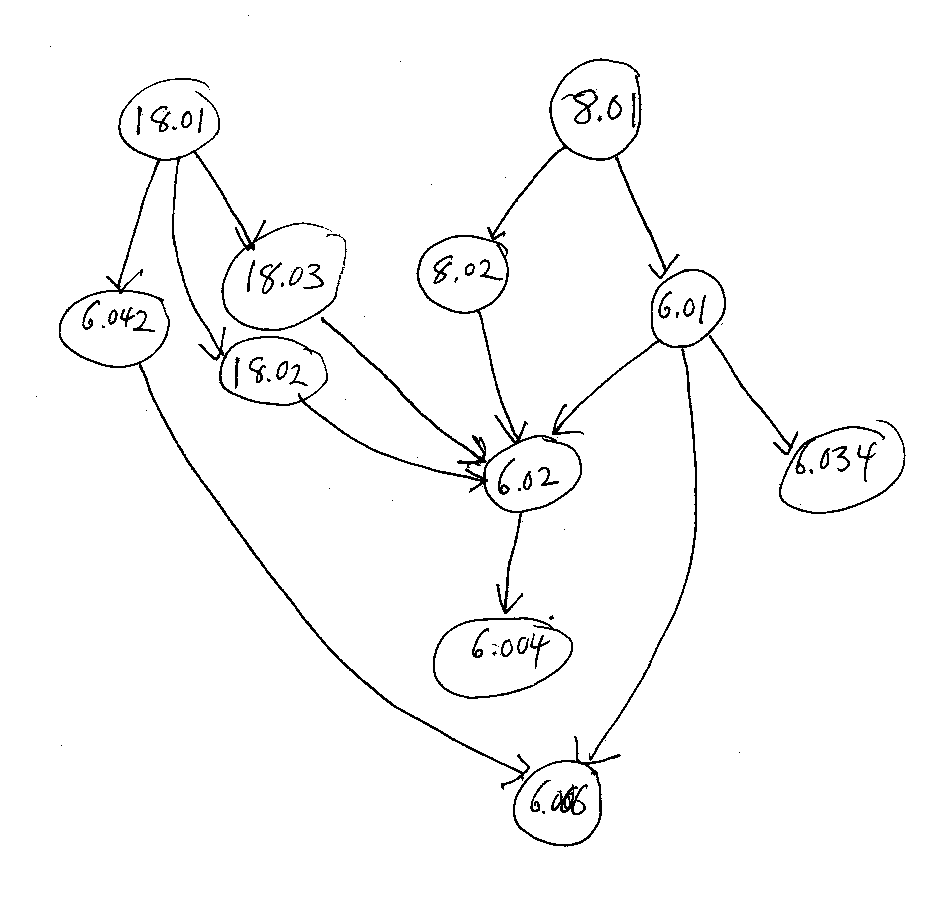
\includegraphics[height=1.5in]{latex-macros/figures/prereq-poset.pdf}
\end{center}\fi


\end{solution}

\eparts

\begin{definition*}
  A binary relation, $R$, on a set, $A$, has the ``same shape'' (is
  isomorphic to) a relation, $S$, on a set $D$ iff there is a
  relation-preserving bijection from $A$ to $D$.  That is, there is
  bijection $f:A \to D$, such that for all $a,a' \in A$,
  \[
  a \mrel{R} a' \qiff f(a) \mrel{S} f(a').
  \]
\end{definition*}

For each of the following binary relations, describe a collection of sets
whose proper subset relation, $\subset$, has the same shape.

\bparts

\ppart the prerequisite relation among MIT subjects from part\eqref{prereqtable}.

\begin{solution}
For each subject, let the corresponding set be the subject itself along
with all the subjects that are indirect prerequisites of that subject.
Remember that a direct prerequisite is considered to be a special case of
an indirect one.

Quickie: What would go wrong if the set corresponding to a subject was only
the indirect prerequisites?  \hint Consider 18.01 and 6.042.
\end{solution}

\ppart  the ``empty'' relation on 5 elements.  That is, the relation
under which no element is related to anything.

\begin{solution}
Choose any 5 sets none of which is contained in any of the others.  For
example, all the size 4 subsets of $\set{1,2,3,4,5}$

\end{solution}

\ppart the "properly contains'' relation, $\supset$, on
$\power{\set{1, 2, 3,4}}$.

\begin{solution}
Let each set $A \subseteq \set{1, 2, 3,4}$ correspond to its
complement.  That is, $f(A) \eqdef \set{1, 2, 3,4} - A$.

\end{solution}

\eparts

\end{problem}

%%%%%%%%%%%%%%%%%%%%%%%%%%%%%%%%%%%%%%%%%%%%%%%%%%%%%%%%%%%%%%%%%%%%%
% Problem ends here
%%%%%%%%%%%%%%%%%%%%%%%%%%%%%%%%%%%%%%%%%%%%%%%%%%%%%%%%%%%%%%%%%%%%%

\endinput
